\competentie
{% competentieformulier
	\competentieformulier
	{% toelichting
		Je hebt kennis en vaardigheden die belangrijk zijn voor
		jouw rol als professional in het ict-werkveld. Je kunt de
		kennis die je hebt opgedaan beoordelen op relevantie.
		Op basis daarvan maak je keuzes bij het uitvoeren en
		oplossen van praktijkvraagstukken. Je hanteert daarbij
		een methodische werkwijze, stelt criteria op waaraan
		het resultaat moet voldoen en werkt volgens
		professionele (internationale) ict-standaarden.
		Je hebt een ondernemende houding.
	}
	{% deelcompetenties
		planmatig werken,
		toepassing van (wetenschappelijke) kennis en inzichten,
		kwaliteit leveren,
		ondernemen
	}
	{%
		Proof
	}
	{%
		Deze competentie wordt beoordeeld door een STARR.
	}
	{% verwijzing naar bewijs
		Figure~\ref{fig:terraform}, 
		Figure~\ref{fig:react},
		Figure~\ref{fig:kubernets},
		Figure ~\ref{fig:terraformcommit}
	}
}
{% bewijzen
	\bewijs
	{% naam
		% TODO 
		Realiseren van de applicatie.
	}
	{% starr
		\starr
		{% betreft
			Kwaliteit leveren,
			ondernemen,
			Planmatig werken
		}
		{% datum
			25-06-2022
		}
		{% situatie
			Een werkgever heeft mij gevraagd een applicatie te realiseren binnen bepaalde een tijd.
			De applicatie moet voldoen aan de gestelde eisen van de werkgever.
		}
		{% taak
			De applicatie moet voldoen aan de gestelde eisen van de werkgever.

			De werkgever heeft geen specificaties gegeven over de techologie die gebruikt moet worden voor de applicatie.

		}
		{% activiteiten
			Voor het realiseren van de applicatie heb ik telefonisch contact gehad om duidelijk te bespreken wat de wensen van de werkgever zijn.

			Op basis van deze criteria kan ik een kwalitatief goede applicatie maken die geschikt is voor de huidige procedure tijdens een spreekuur.

			Omdat de klant niet een specifieke techologie heeft aangegeven heb ik het risico genomen om de applicatie met techologien te maken waar ik zelf nog niet bekwaam mee ben.

			Voor het realiseren van de applicatie ben ik planmatig begonnen met het bestuderen en leren van de inhoud van de cursussen.
			Met deze kennis heb ik daarna de applicatie gerealiseerd.

			Door correct gebruik te maken van kubernetes is het mogelijk het project snel en effiecient te updaten met minimal downtime.

		}
		{% resultaat
			Het resultaat is een applicatie die kan schalen naar gebruik van de user en voldoet aan de vooraf gestelde eisen van de werkgever.

			De applicatie kan snel worden geupdate door gebruik te maken van de techologie en hier correct mee om te gaan.
			De applicatie kan grote hoeveelheid verkeer aan dankzij kubernetes.
			Met deze techologie is de applicatie in staat snel op te schalen om zo meer verkeer te kunnen verwerken.

			Door het risico te nemen om nieuwe techologien te gebruiken ben ik nu ook bekwamer bij mijn huidige werkgever dankzij de nieuwe kennis.
		}
		{% reflectie

			Het kiezen voor Kubernetes en terraform heeft het nodig stress geleverd.
			Vooral Kubernetes was erg complex.

			Door planmatig te werken en op tijd te beginnen met het verwerken en leren van de cursussen heb ik genoeg tijd gehad om de applicatie op tijd te kunnen realiseren.

			Het heeft veel tijd gekost om op een correcte manier gebruik te maken van Kubernetes.
			Dit kwam omdat er veel nieuwe methodieken werden geintroduceerd die allemaal met elkaar moeten samen werken.

			Het composeren van alle losse individuelen delen zoals de load balancer, service en applicatie zelf heeft tijd gekost.

			Ook is het niet gelukt terraform te gebruiken in dit project.
			Ik gebruik dit wel actief bij mijn huidige werkgever met de nieuw behaalde kennis.


			De reden dat het niet gebruikt is in deze applicatie heeft te maken met een verkeerde interpetatie van de techologie.
			Terraform wordt gebruikt voor het managen van cloud componenten en niet voor het managen van een single applicatie.

			Doordat ik in eerste instantie een verkeerd beeld had van het gebruik van Terraform, heb ik hier veel van geleerd.
		}

		{
		}
	}
	{% bewij
		\begin{figure}[H]
			\begin{center}
				
\includegraphics[width=0.95\textwidth]{images/terra.jpg}
			\end{center}
			\caption{Terraform}
			\label{fig:terraform}
		\end{figure}
		\begin{figure}[H]
			\begin{center}
				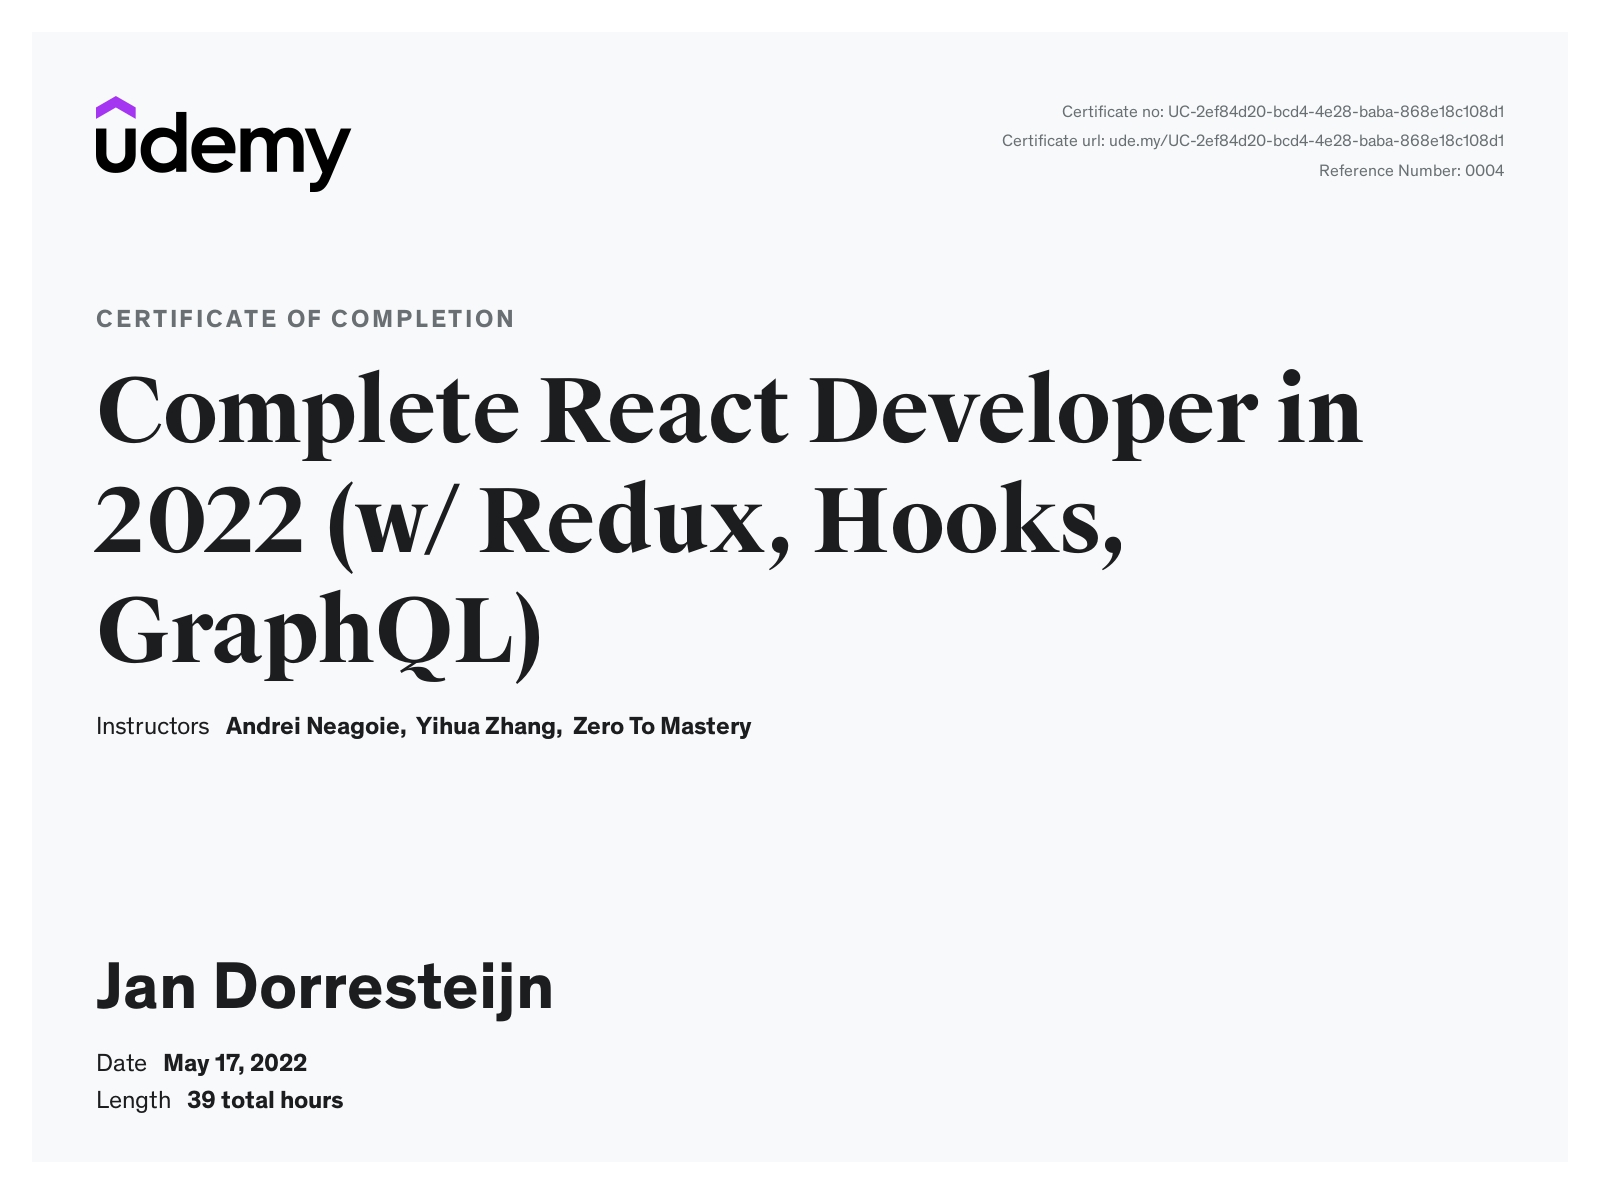
\includegraphics[width=0.95\textwidth]{images/react.jpg}
			\end{center}
			\caption{React}
			\label{fig:react}
		\end{figure}
		\begin{figure}[H]
			\begin{center}
				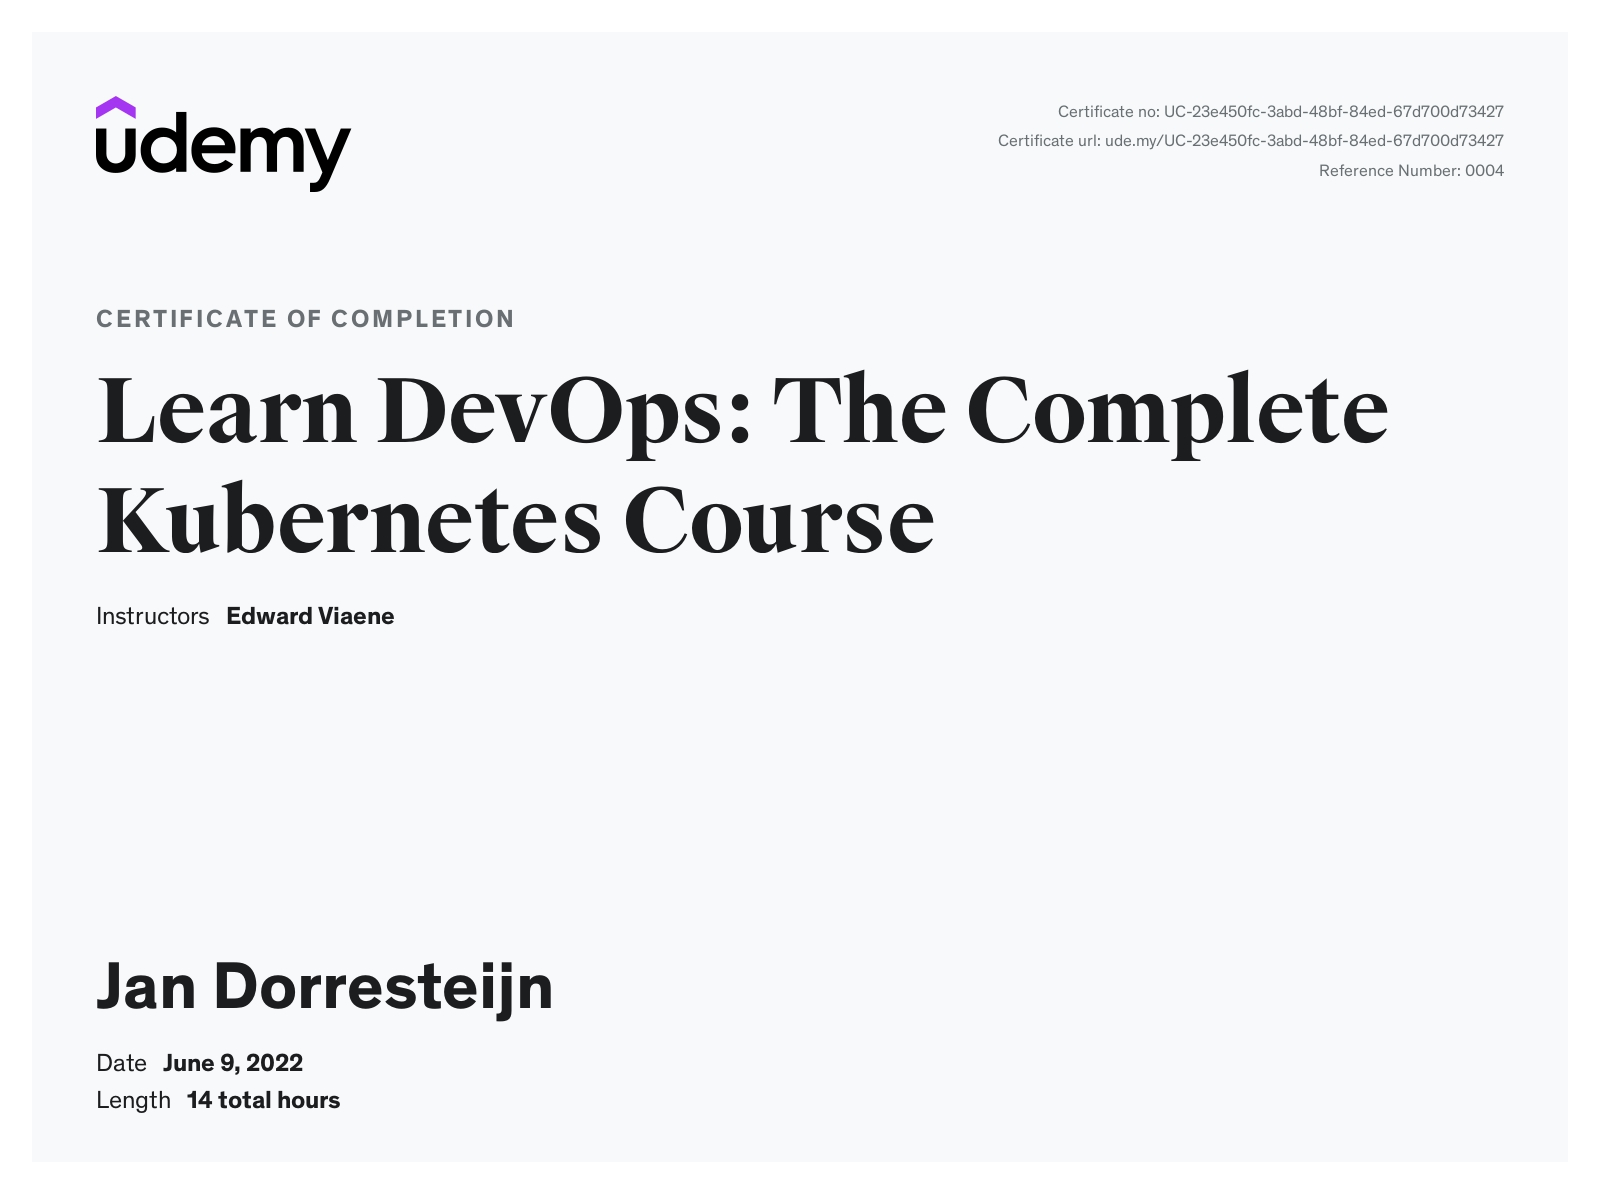
\includegraphics[width=0.95\textwidth]{images/kube.jpg}
			\end{center}
			\caption{Kubernetes}
			\label{fig:kubernets}
		\end{figure}

	},
	\bewijs
	{% naam
		Beter onderzoek doen naar de tools die ik wil gebruiken.
	}
	{% starr
		\starr
		{% betreft
			Planmatig werken
		}
		{% datum
			25-06-2022
		}
		{% situatie
			Voor het realiseren van de applicatie had ik bepaalde techologien willen gebruiken.
			Deze techologien heb ik aangegeven een cursus voor te doen om ze daarna te kunnen toepassen in een echte situatie.
			\begin{itemize}
				\item Kubernetes
				\item Terraform
				\item React
			\end{itemize}
		}
		{% taak
			Om deze techologien te gebruiken moest ik de cursussen afmaken en vervolgens toepassen voor de applicatie.
		}
		{% activiteiten
			Ik ben begonnen met react omdat het ontwikkelen van de back-end en front-end de eerste stappen zijn .

			Toen de basis van de applicatie klaar was ben ik begonnen met het implementeren van de deployment stappen.
			Met kubernetes is het duidelijk wat ik moest doen en is het mij gelukt dit te realiseren met de applicatie.
			Voor Terraform had ik een verkeerde interpretatie wat de techologie doet en waar het gebruikt voor wordt.

			Ik heb uiteindelijk terraform niet gebruikt bij deze applicatie.

		}
		{% resultaat
			Omdat ik van te voren niet genoeg onderzoek heb gedaan naar de gekozen techologien kon ik mijn plan niet waarmaken.

			Ik was van plan Terraform te gebruiken voor netwerk verkeer, omdat ik dacht dat Terraform hiervoor gebruikt wordt.

			Pas bij het daadwerkelijk leren van de techologie kwam ik er achter dat het een compleet andere toepassing heeft die niet relevant is voor de huidige applicatie.
		}
		{% reflectie

			Ik had een beter initieel idee nodig over hoe en waarom een techologie gebruikt wordt.
			Ik had dit beter planmatig kunnen aanpakken door een beter vooronderzoek te doen naar het gebruik van.

			Gelukkig kan ik de kennis wel gebruiken bij mijn huidige werkgever.
			Ik heb deze kennis bijvoorbeeld gebruikt bij het maken van een automatisch ddl mechisme dat een time serie database op verschillende ontwikkelings omgegevingen maakt.

			Dit had ik niet gekund zonder de kennis die ik heb verkregen tijdens de cursus.
		}
		{
		}
	}
	{% bewij

		\begin{figure}[H]
			\begin{center}
				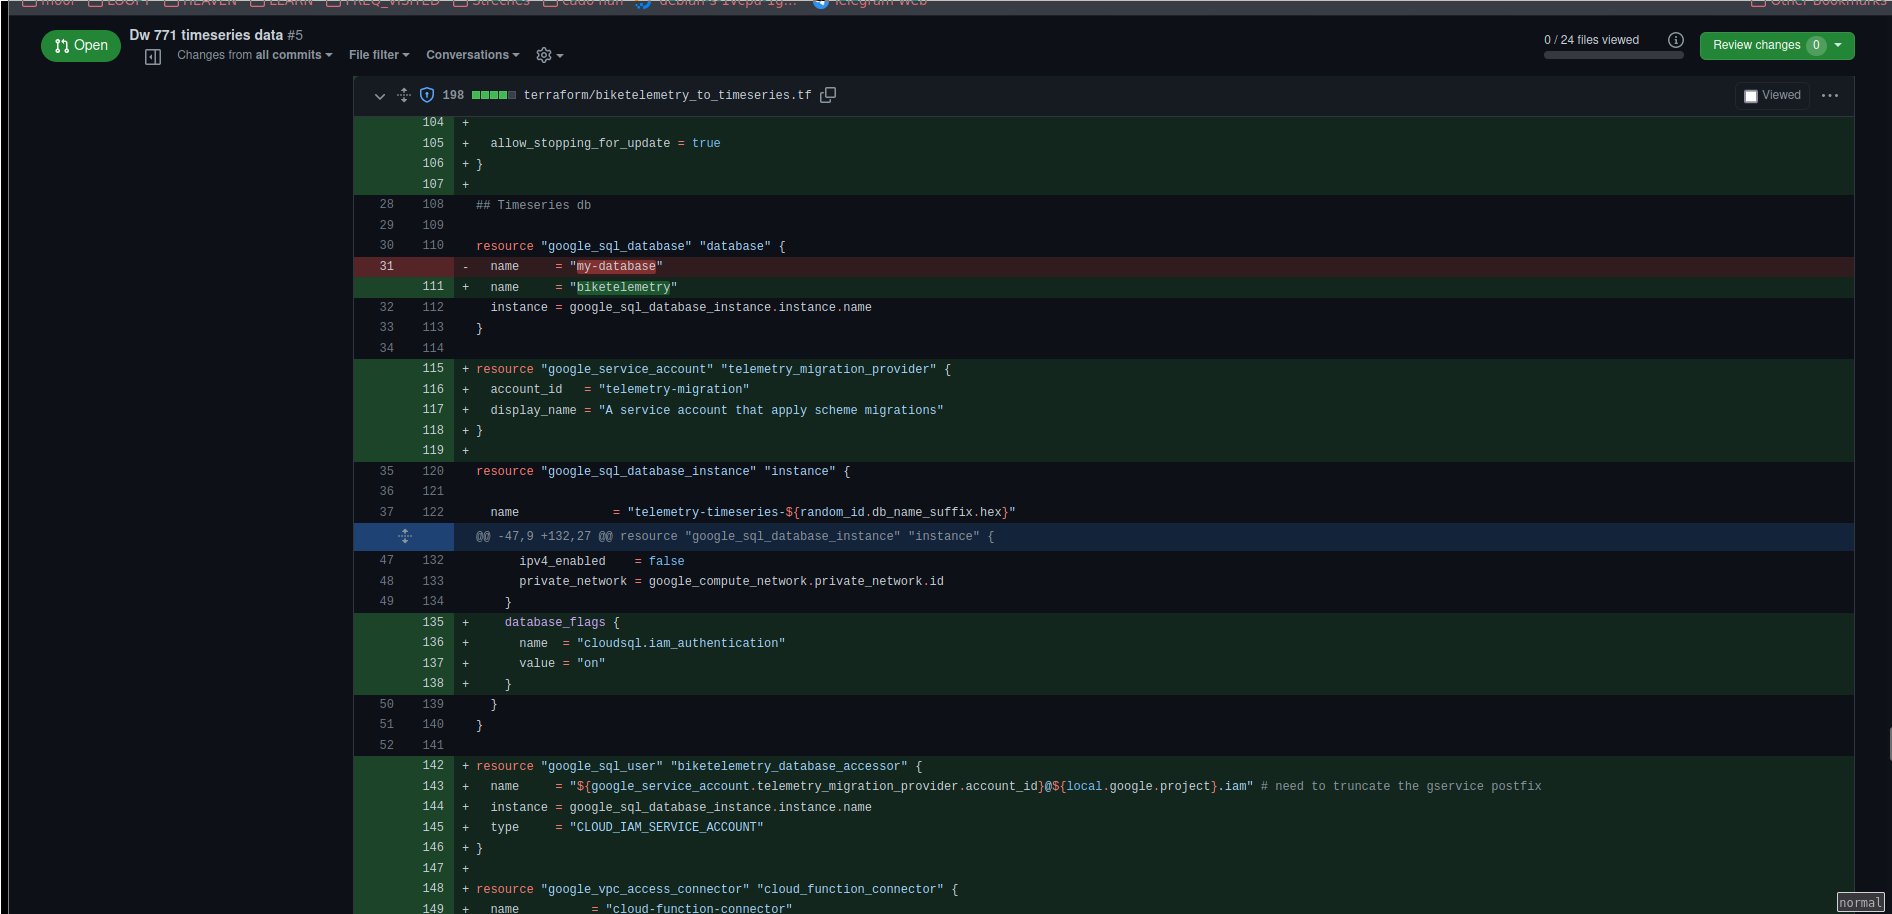
\includegraphics[width=0.95\textwidth]{images/timeseries.png}
			\end{center}
			\caption{Een git contributie aan een Terraform commit voor een timeserie database voor VanMoof}
			\label{fig:terraformcommit}
		\end{figure}

	},
}

